\documentclass[11pt,a4paper]{scrbook} 
\usepackage[utf8]{inputenc}
\usepackage{amsmath}
\usepackage{amsfonts}
\usepackage{amssymb}
\usepackage{graphicx}
\usepackage{longtable}
\usepackage{multirow}
\renewcommand{\familydefault}{\sfdefault}
\usepackage{droid}
\usepackage[left=2cm, right=2cm, top=1cm, bottom=2.5cm]{geometry}
\usepackage{ngerman}
\usepackage{tabularx}
\usepackage{graphicx}
\usepackage{enumitem}
\usepackage{scrpage2}	%Kopf- und Fußzeile
\usepackage{picinpar}	%Textumläufe von Grafiken
\usepackage{pdfpages}	%Implementierung von pdf als ganze Seite(Seiten sind nicht editierbar)
\usepackage{lastpage}	%Implmentiert 'letzte Seite', wird für Kopfzeile benötigt
\usepackage{listings}
\usepackage{tikz}
\usepackage{wasysym}  
\usepackage{lastpage}


\pagestyle{scrheadings}

\ifoot{\ \copyright Noah Kofort, Klaus Suthe - v1.0} \setfootsepline{1pt}\ofoot{ \thepage \  von \pageref{LastPage}\ }



\begin{document}

\raggedleft
\includegraphics[height=1.5cm]{images/hbbk-logo.png}
\\
\begin{tabular}{p{4cm} p{5cm} p{1.5cm} p{1.5cm} p{3cm}}
  \tabularnewline
  \textbf{GK Informatik} & \textbf{Projekt GIACar}    & GIA3    &  & {\today} \tabularnewline 
  \hline
\end{tabular}


\centering
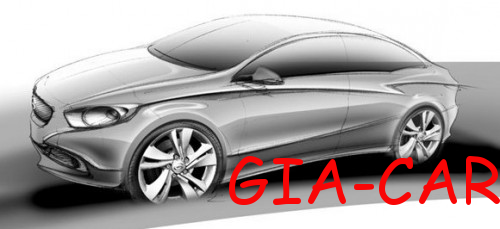
\includegraphics[width=0.7\linewidth]{./images/GIAcar}

\centering\Huge{Lastenheft} \\

\flushleft
\normalsize

\section*{Ausgangssituation}
Nachdem die GIA-Car AG 
jahre lang in Preis und Leistung überzeugt hat, soll nun der
nächste technologische Fortschritt geschaffen werden. Die Idee Autos automatisierter und anwenderfreundlicher zu 
verkaufen stand schon lange im Raum, ist aber erst jetzt zur
Umsetzung bereit. Das Problem war, dass die Angebote nicht die ganze Zielgruppe erreicht haben und dadurch fehlende Umsätze nicht entstanden sind. In der Vergangenheit wurde lange nach einer Möglichkeit gesucht das Angebot zu erweitern, doch erst jetzt haben wir die nötige Kooperation mit einem IT-Unternehmen gefunden, welche unseren Ansprüchen
gerecht werden kann.

\section*{Zielsetzung}
Verkaufssteigerung soll erreicht werden durch
\begin{itemize}
\item Benutzerfreundlichkeit
\item individuelle Kundenangebote
\item Kundenanalyse
\item mehr Kunden erreichen / Reichweite
\item möglichst barrierefreier Kauf/Verkauf
\end{itemize}

\section*{Produkteinsatz}
Onlineshop im Internet


\section*{Funktionale Anforderungen}
\begin{itemize}
\item Fahrzeugverwaltung:
	\begin{itemize}
	\item Fahrzeuge hinzufügen, löschen, modifizieren, lokalisieren, allgemeine Informationen, Preis, Bilder
	\item Bewertungssystem
	\end{itemize}
\item Verkauf: 
	\begin{itemize}
	\item Angebote
	\item Aktionen und Angebotskampagnen  erstellen
	\item Versteigerungssystem
	\item Kundenverwaltung mit der Möglichkeit, Angebote für den Kunden zu finden und ihm per Klick anzubieten.
	\item Angebot auf der Grundlage des letzten Kaufs $\rightarrow$ z.B.: Angebot eines neuen Wagens, wenn der letzte ein bestimmtes Alter erreicht hat.
	\end{itemize}
\item Kundenportal: 
	\begin{itemize}
	\item Übersichtlich, Such- und Filterfunktion, Kontaktdaten
	\item Individualisierte Startseite
	
	\end{itemize}
\item Kunden und Sachbearbeiterverwaltung
\item Impressum, rechtliche Informationen, Nutzungsbedingungen/allgemeine Geschäftsbedingungen
\item Dokumentation, Installation und Einweisung

\end{itemize}

\section*{Nichtfunktionale Anforderungen}
\begin{itemize}
\item ansprechendes Design
\item intuitive Bedienung/Zugang
\end{itemize}

\section*{Lieferumfang}
\begin{itemize}
\item Software
\item Support
\item Dokumentation
\item Server mit der Verkaufsplattform
\end{itemize}

\section*{Phasenplanung}

Diagramme $\longrightarrow$ Server $\longrightarrow$ Design $\longrightarrow$ Funktionen planen $\longrightarrow$ Datenbanken $\longrightarrow$ Funktionen $\longrightarrow$ Versionsmanagment


\section*{Offene Punkte, die noch zu klären sind}
\begin{itemize}
\item Rechnungsausstellungen
\end{itemize}

\section*{Abnahmekriterien und Qualitätsanforderungen}

\begin{itemize}
\item Fehlerfreie und einwandfreie Software
\end{itemize}




\end{document}
